% main.tex
\documentclass[12pt]{article}

% Import formatting & packages
% preamble.tex
\usepackage[a4paper, margin=2.5cm]{geometry}  % Page size & margins
\usepackage{graphicx}   % Figures
\usepackage{booktabs}   % Professional tables
\usepackage{amsmath}    % Math symbols & equations
\usepackage{amssymb}    % More math symbols
\usepackage{hyperref}   % Hyperlinks
\usepackage{cleveref}   % Smart references
\usepackage{enumitem}   % Customizable lists
\usepackage{float}      % Better table/figure placement
\usepackage[utf8]{inputenc}  % Ensure Overleaf uses UTF-8 encoding
\usepackage{csquotes}   % Improved quotation formatting
\usepackage{tabularx}
\usepackage{tabularray}
\usepackage{tikz}
\usetikzlibrary{shapes.geometric, arrows}
\usepackage{pgfplotstable,siunitx,xfp}
\pgfplotsset{compat=1.18}
\usepackage{siunitx}   % \num, rounding/formatting
\usepackage{xfp}       % or expl3; xfp gives \fpeval
\usepackage{titling} 
\usepackage{verbatim} % for \verbatiminput
\usepackage{catchfile}
\usepackage{multirow}
\usepackage{booktabs}
\usepackage{array}
\usepackage{setspace}


% Bibliography
\usepackage[backend=biber, style=authoryear, sorting=nyt]{biblatex}  
\addbibresource{references.bib}  % Link to your Zotero export

% Section number depth
\setcounter{secnumdepth}{3}

% Table & figure captions
\usepackage[labelfont=bf]{caption}  

 % Word count command
\newcommand{\wordcount}{%
  % Run texcount on the main document (jobname.tex)
  %  - stdout -> \jobname.wc
  %  - stderr (warnings) -> nul (ignored)
  \immediate\write18{texcount -inc -sum -0 -template={SUM} \jobname.tex > \jobname.wc 2> nul}%
  % Read the result from the temporary file:
  \CatchFileDef{\wcresult}{\jobname.wc}{}%
  \mbox{\wcresult\unskip}%
}









\begin{document}

%TC:ignore
\begin{titlepage}
  \begin{center}
    \vspace*{1cm}

    % University + document type
    {\Large UNIVERSITEIT UTRECHT\par}
    \vspace{0.5cm}
    {\large MASTER THESIS\par}

    \vspace{2cm}

    % Title
    {\Huge \textbf{Jump-Starting Evidence Synthesis}\par}
    \vspace{0.5cm}
    {\LARGE
      Initializing Active Learning Models for Systematic Reviews using LLM-generated Data \par
    }

    \vspace{2.5cm}

    % Author(s)
    {\large \textbf{Author:}\par}
    \vspace{0.2cm}
    {\large Timo van Ommeren\par}

    \vspace{1cm}

    % Supervisor(s)
    {\large \textbf{Supervisors:}\par}
    \vspace{0.2cm}
    {\large Prof. dr. A.G.J. (Rens) van de Schoot, Lauke Stoel\par}

    \vspace{1.5cm}

    % Programme / degree line (adapt as you like)
    {\large
      MSc Methodology and Statistics for the Behavioural,\\
      Biomedical and Social Sciences\par}

    \vspace{0.5cm}

    % Host department / organisation (mirroring "Ministry of Health..." line)
    {\large Methodology Department, Utrecht University\par}

    \vfill

    % Logo
    \includegraphics[width=0.2\textwidth]{images/Utrecht_University.png}

    \vspace{0.8cm}

    % Date and word count
    {\large \today\par} {\large Word count: \wordcount}

  \end{center}
\end{titlepage}
%TC:endignore


\section{Introduction}

\subsection{Background}

\subsubsection{Active Learning Models for Systematic Reviewing}

Researchers and practitioners are continually challenged to base their decisions on the latest scientific evidence. Systematic reviews and meta-analyses were developed to address this need as rigorous methods of summarizing scientific literature \parencite{chalmers2002brief, bastian2010seventy}. However, systematically reviewing the literature can be time-consuming, which limits its practical applicability, especially, in, for example, times of crisis \parencite{tricco2020rapid, nussbaumer2021resource}.

Fortunately, recent advances in machine learning have produced tools that allow for the systematic screening of scientific literature while greatly reducing the need for manual screening \parencite{van2021open}. Specifically, active learning models (ALMs) ask users to screen titles and abstracts of papers one by one. Based on the user's decision, the models reassess the probability that the remaining papers are relevant and thus whether to show them to the user. In other words, these models continually reshuffle the papers retrieved from a scientific literature search based on the user's interests. This method reduces the time needed to find as many relevant papers as possible compared to simple index-based screening \parencite{van2025hunt}. 

\subsubsection{The Cold Start Problem}

A key challenge to using active learning for systematic reviews is that these models face a "cold start" \parencite{panda2022approaches}. For an ALM to query a user with a potentially interesting paper, the model must first have knowledge of the user's interests . One way of overcoming a cold start is to initialize, or 'warm up', the ALM using examples of relevant and irrelevant papers \parencite{teijema2025large}. If however no examples are available the user may simply start screening 'from the top-down', until a relevant and an irrelevant paper have been found. 

\subsubsection{The Advent of Large Language Models}

With the recent advent of large language models (LLMs), a new possible solution to overcoming the cold start problem has emerged \parencite{bachmann2025adaptive}. It may be advantageous to prompt an LLM with the inclusion and exclusion criteria of a systematic review to generate synthetic examples of relevant and irrelevant papers. And initialise the ALM using these examples, rather than screening from the top-down until actual examples are found. This may be particularly true if the percentage of relevant papers obtained from a systematic search is rather low. In this case, active learning assisted screening using even a sub-optimal example of a relevant paper may be preferable to random screening for hundreds or thousands of papers. That said, the use of synthetic data may also misdirect the ALM by contaminating the model's training data. 

It may therefore be possible to overcome the cold start problem and improve starting performance by using LLMs to generate examples of relevant and irrelevant papers to initialize the ALMs for systematic reviews. This approach could be particularly useful if a user has no relevant examples available, as it avoids top-down screening. However, using synthetic data generated by LLMs seems less likely to improve starting performance if a user has access to actual examples. A key question is whether the LLM-generated examples improve starting performance over and above initialisation using the inclusion and exclusion criteria of the systematic review.

\subsection{Statistical Framework}

% \subsubsection{Generalized Linear Mixed Models for discrete proportion data}

% Defining residual variance for non-gaussian models is non-trivial. One way of definining residual variance is as 1 minus the ratio of the maximum likelihood of the current model and the null model. This definition, however, can become problematic when extended to non-gaussian mixed models, in part because likelihoods cannot be compared when using restricted maximum likelihood estimation (REML) \parencite{nakagawa2013general, stroup2024generalized}. Similarly, the intraclass correlation coefficient (ICC), which quantifies the proportion of variance explained by grouping structure in mixed models, is not straightforward to compute for non-gaussian models \parencite{nakagawa2017coefficient}. One solution is to de-couple the meand and variance using a variance-stabilizing transformation \parencite{nakagawa2010repeatability}.

% There are no established REML methods for non-gaussian mixed models \parencite{maestrini2024restricted}. One way of dealing with this is to use maximum likelihood estimation (ML) instead. However, ML estimates of variance components may be biased downwards. Another solution is to use Bayesian methods, which do not rely on ML or REML.



\subsubsection{Data generating process 1: AI-assisted screening}

\parencite{agresti2002categorical}

The starting performance of AI-assisted systematic reviews can be evaluated by simply counting the number of relevant papers successfully retrieved from a given number of screened papers (i.e., X out of n, with $n \leq 100$ trials). In other words, we may discount the fact that the true data generating process (DGP) is a dynamic sequence, and consider starting performance as a discrete proportion of successes from independent trials. This simplifying assumption allows for the application of generalized linear models (GLMs), specifically the binomial model \parencite{nelder1972generalized}. 

The main issue with applying a binomial model to a dynamic sequence is that, in contrast to assumed independent Bernoulli trials, a successful retrieval increases the probability of subsequent successes, and vice versas\footnote{%TC:ignore
The DGP of AI-assisted screening can be seen as analogous to the Pólya urn problem, in which each time a ball of a certain colour is drawn, an additional ball of the same colour is added to the urn ('the rich get richer'; \cite{eggenberger1923uber, kotz2000generalized}). Notably, the beta-binomial model can be derived from Pólya's urn model \parencite{helfand2013polya}.}. %TC:endignore 
This reinforcement mechanism leads to dependence between trials which increases the variance in the number of successes compared to what would be expected under a binomial model, which manifests as overdispersion. One way of dealing with overdispersion is to use a beta-binomial model \parencite{skellam1948probability, harrison2015comparison, kim2017validation}. The beta-binomial is generalized linear mixed model (GLMM) in which the probability of success is a random variable that follows a beta distribution \parencite{stroup2024generalized}. Formally, the beta-binomial model can be defined as follows:

\begin{equation}
X_i | p_i \sim \text{Binomial}(n_i, p_i) \quad \text{with } p_i \sim \text{Beta}(\alpha_i, \beta_i)
\end{equation}

For interpretability, we reparamterize $\alpha_i$ and $\beta_i$ in terms of the beta mean, $\mu_i$, and precision, $\phi_i$:

\begin{equation}
p_i \sim \text{Beta}(\mu_i \phi_i, (1 - \mu_i)\phi_i) \quad \text{with } \mu_i = \frac{\alpha_i}{\alpha_i + \beta_i} \quad \text{and} \space \phi_i = \alpha_i + \beta_i
\end{equation}

This reparametrisation further clarifies how modelling can work using the beta-binomial model \parencite{stroup2024generalized}. For example, the mean parameter $\mu_i$ can be modelled using a GLM, while the precision parameter $\phi_i$ can be used to either simply control for overdispersion (i.e., a single precision parameter for all observations) or to model heterogeneity in overdispersion (i.e., different precision parameters for different groups of observations).

\subsubsection{Data generating process 2: random sampling due to a cold start}

In reality, two DGP are at play in AI-assisted systematic reviews. The first is AI-assisted screening, which takes place once the AI has been trained using relevant and irrelevant titles and abstracts. However, in the cold-start condition, screening must be done at random until at least one relevant and one irrelevant paper have been identified. This may result in runs where no relevant papers are found. These 'structural zeros' may be considered to come from a different DGP. One way to address this issue is to use zero-inflation models \parencite{lambert1992zero, wagner2015importance}. 

\subsubsection{Multilevel structure: clustering by dataset}

Finally, starting performance may vary systematically between datasets due to differences in topic, percentage of relevant papers return by search, and abstract style, for example \parencite{de2023synergy}. One way of dealing with differences between datasets is to add dataset as a covariate to the model. However, since we are not interested in the effect of specific datasets per se, it may make more sense to treat dataset-specific variations as the results of a random variable. In other words, we may treat dataset as a random effect in a generalized linear mixed model (GLMM) (see Chapter 1 of \cite{stroup2024generalized} for when GLMMs are appriopriate).

\subsection{Objectives}

This study aims to investigate the effect of using LLM-generated data to initialise active learning models (ALMs) for systematic reviews, compared to random initialisation, no initialisation or criteria-based initialisation, on starting performance. This will be achieved by simulating the screening of previously published systematic reviews.

% The aim is to investigate the effect \textit{on starting performance} of initializing  ALMs for systematic reviews using:
% \begin{enumerate}[label=\arabic*), leftmargin=*, nosep]
%     \item examples of relevant and irrelevant papers generated by LLMs;
%     \item examples of relevant and irrelevant papers randomly sampled from the sets of screened papers;
%     \item without any examples,
% \end{enumerate}

\section{Methodology}

\subsection{Simulation set-up}

In order to investigate the effect of LLM initialisation, random initialisation, no initialisation or criteria-based initialisation on starting performance, the SYNERGY datasets will be screened based on the abstracts and titles of the papers using ASReview's ALM. ASReview is an open-source software package for semi-automated systematic reviewing that implements several ALMs. To simulate the screening process, we will access ASReview via its Python API. For all simulation runs, we will use the recommended U4 configuration in ASReview, which combines a support vector machine classifier with a bi-gram term-frequency inverse document frequency (TF-IDF) feature extractor. The SYNERGY datasets consist of 26 previously screened and labelled sets of papers. Importantly, this gives us access to the ground truth labels of all the papers in these datasets. See Appendix \ref{tab:SYNERGY} for a list of all datasets including their topic, total number of records, number of records included and the percentage of relevant records \parencite{de2023synergy}. 

For each run, the simulation makes use of two ALMs. The first ALM consists of only a random sampler which runs until a fittable training set (of at least one relevant and one irrelevant paper) is obtained. Note however that depending on the condition an example of a relevant paper(s) may already have been provided prior to the first ALM. The second ALM then initialised using the examples obtained from the first ALM and the examples provided prior to the first ALM. The parameters of the second ALM are then set to the recommended U4 configuration in ASReview. See figure \ref{fig:sim-pipeline} for a schematic of the simulation pipeline. The classifier is seeded with the run number. 

See exact code: \href{https://github.com/timovanommeren/thesis_timo/blob/main/simulations/simulation.py}{here}


\hspace{1cm}

\begin{figure}[htbp]
  \centering
    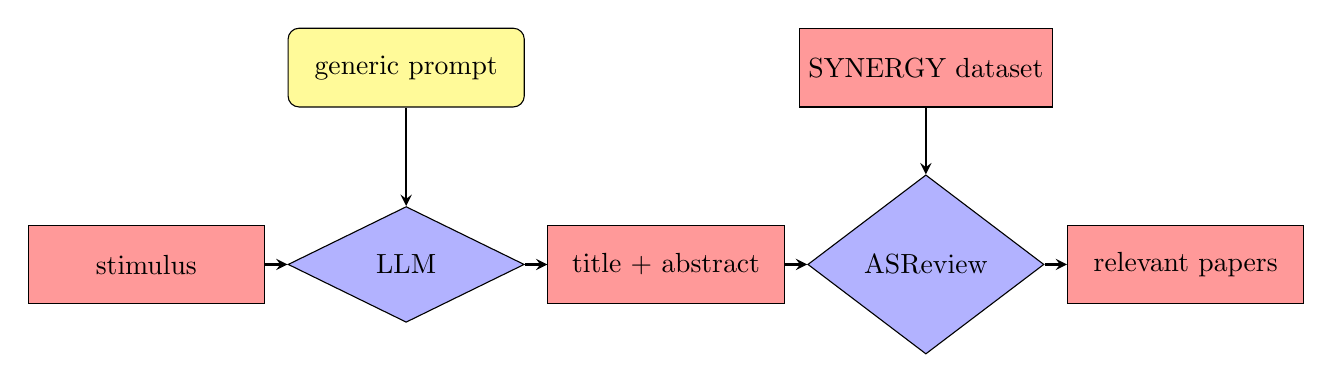
\begin{tikzpicture}[node distance=2.5cm]
    
    \tikzstyle{data} = [rectangle, minimum width=3cm, minimum height=1cm,text centered, draw=black, fill=red!40]
    \tikzstyle{prompt} = [rectangle, rounded corners, minimum width=3cm, minimum height=1cm,text centered, draw=black, fill=yellow!40]
    \tikzstyle{process} = [diamond, minimum width=3cm, minimum height=1cm, text centered, draw=black, fill=blue!30]
    \tikzstyle{arrow} = [thick,->,>=stealth]
    
    % \tikzstyle{io} = [trapezium, trapezium left angle=70, trapezium right angle=110, minimum width=3cm, minimum height=1cm, text centered, draw=black, fill=blue!30]
    % \tikzstyle{process} = [rectangle, minimum width=3cm, minimum height=1cm, text centered, draw=black, fill=red!30]
    
    \node[data]    (stim) {stimulus};
    \node[process, right of=stim, xshift=0.8cm] (llm) {LLM};
    \node[prompt,    above of=llm]  (prom)  {generic prompt};
    \node[data,    right of=llm, xshift=0.8cm]  (ta)  {title + abstract};
    \node[process, right of=ta, xshift=0.8cm]   (asr) {ASReview};
    \node[data,    above of=asr]  (syn)  {SYNERGY dataset};
    \node[data,    right of=asr, xshift=0.8cm]  (rel) {relevant papers};
    
    \draw[arrow] (stim) -- (llm);
    \draw[arrow] (prom) -- (llm);
    \draw[arrow] (llm)  -- (ta);
    \draw[arrow] (ta)   -- (asr);
    \draw[arrow] (syn)   -- (asr);
    \draw[arrow] (asr)  -- (rel);
    
    \end{tikzpicture}
    \caption{Simulation pipeline (for more detailed schematic of workings within ASReview see \parencite{asreviewvs2jonathan})}
  \label{fig:sim-pipeline}
\end{figure}

\subsection{Conditions}

This study aims to compare the effect of LLM initialisation (the experimental condition) to three control conditions (random initialisation, no initialisation, and criteria-based initialisation). 

\subsubsection{LLM initialization}

In the LLM initialisation condition, the ALM's classifier is provided with a set of examples comprising at least one relevant and one irrelevant paper before screening is simulated. These examples are generated based on the inclusion and exclusion criteria of the given systematic review publication. See figure \ref{fig:sim-pipeline} for a schematic of the simulation pipeline. 

Between simulation runs the exact number of abstracts generated as well as their specific contents is varied. More specifically, we aimed to investigate the effect of the following variables on starting performance: 
\begin{enumerate}[label=\arabic*)]
\item degree of information provided to the LLM about the systematic review in question \textbf{(3 levels)}, 
\item number of abstracts generated per simulation run \textbf{(4 levels)},
\item length of abstracts generated per simulation run \textbf{(4 levels)},
\item typicality of abstracts generated per simulation run \textbf{(5 levels)},
\item the use of jargon in generated per simulation run \textbf{(5 levels)}.
\end{enumerate}

More specifically, the LLM was provided with either: (a) the title of the published systematic review, (b) the inclusion and exclusion criteria of the systematic review, or (c) the abstract of the published systematic review. Number of abstracts was varied between 1-2-5-10 abstracts per run. The length was varied between 100-200-500-1000 words per run. Whether the abstract should be a typical example of a paper in this review or rather an edge case was varied if 5 or 10 abstracts were generated. In this case the ratio between typical and atypical examples was varied between 00-20-40-60-80-100 \% typical. Finally, the use of jargon was varied similarly to typicality by generating abstracts which were simply pure lists of jargon and combining these with regularly written abstract in  the ratio 00-20-40-60-80-100 given that at least 5 or 10 abstracts were generated. 

To instruct the LLM, a DSPY module was created which takes the variables described above as input, as well as whether the abstract should be relevant or irrelevant \parencite{khattab2023dspy}. Note that to generate multiple abstracts per run, the module was simply looped over and called multiple times. For the exact code, see: \href{https://github.com/timovanommeren/thesis_timo/blob/main/simulations/prompting.py}{here}

\subsubsection{Random initialization}

In the random initialization condition, one relevant and one irrelevant paper were randomly sampled prior to the start of screening. An ALM could therefore be used starting from the very first paper screened. 

\subsubsection{No initialization}

In the no initialisation condition, no papers were provided prior to the start of screening. Therefore, two separate ALMs were used to simulate the screening process. The first ALM randomly sampled papers until at least one relevant and one irrelevant paper were found. These papers were then used to initialise a second ALM, which was used to screen the remaining papers.

\subsubsection{Criteria-based initialization}

Finally, in the criteria-based initialisation condition, the eligibility criteria of the systematic review were directly used as an example of a relevant paper to initialize the ALM. This condition thus serves as a control condition to investigate whether the LLM adds any information over and above the eligibility criteria. 
\subsection{Outcome variable}

\subsubsection{Starting performance}

Starting performance will be assessed based on the number relevant papers in the first 100 papers screened. This figure is derived from research showing that approximately 100 papers can be screened in an hour \parencite{nussbaumer2021resource}. For each simulation, we count the number of relevant records found with a \textit{Time to Discovery} below 100 for each simulation \parencite{ferdinands2023performance}.

\subsection{Data Generation and Analysis}

\subsubsection{Padding}

It is important to note that the simulation may stop prematurely if all the relevant records are found before the desired stopping rule is reached (e.g. screening 100 records). In order to accurately emulate a researcher who is unaware that all the relevant records have been found and who therefore continues to screen until the stopping rule is reached, the simulation results were appended with rows containing the label 'zero' (i.e. irrelevant records). The number of these rows is determined by taking the number of records that should have been screened (the stopping rule) minus the number of records that were screened (in the random initialisation condition the number of records that were provided prior to screening is also subtracted). This is referred to as padding and ensures that the final simulation results are accurate.

\subsubsection{Recall plots}

A common way of visualizing the simulation results of retrieval tasks in general, and systematic reviews in particular, are recall curves. These curves shows the number of relevant records retrieved at a given number of papers screened. At the end of each simulation run, a recall plot is created containing three curves: one for each condition. Furthermore, at the end of the entire simulation study, an aggregate recall plot is created per dataset, containing the average recall curve of each condition, as well as it's standard error between runs. 

\subsubsection{Exported results}

Each simulation run is stored in a separate CSV file. Every row represents a screened paper and contains the following information:

\begin{enumerate}[label=\arabic*), leftmargin=*, nosep]
  \item The paper's record ID,
  \item The assigned label (i.e., relevant or irrelevant),
  \item The classifier, querier, balancer and feature extractor used,
  \item The size of the training set,
  \item A time tag.
\end{enumerate} 

Furthermore, the following naming convention is used for the CSV files: \newline condition\_run\_run\_IVs\_n\_abstracts\_length\_abstracts\_typicality\_degree\_jargon\_llm\_temperature.csv. The same naming convention is used for the recall plots of each simulation run and for the generated abstracts in the LLM initialisation condition.

Finally, at the end of each run, the current values of the input parameters, the outcome variables and other relevant metadata are appended to a long format master dataframe for analysis. The columns of this dataframe are as follows:

\begin{enumerate}[label=\arabic*), leftmargin=*, nosep]
    \item the name of the outcome variable
    \item the value of the outcome variable
    \item name of the simulated dataset,
    \item the condition,
    \item the values of the independent variables:
        \begin{enumerate}
        \item number of abstracts
        \item length of the abstracts
        \item temperature settings of the llm (i.e., diversity)
        \end{enumerate}
    \item timestamp
    \item the run number
\end{enumerate}

This yields a data-frame containing one observation for each combination of dataset (n=26), condition (n=3), independent variables and their levels (n=$3 \times 4 \times 4 \times 5 \times 5 = 1200$), and run (n=1), thus with $26 \times 3 \times 1200 \times 1 = 93600$ rows, and the 12 columns enumerated above. 


\subsubsection{Analysis}

The majority of the variance in the number of relevant records found in the first 100 screened is expected to be explained by differences between datasets. We would therefore like to seperate within-dataset variance from between-dataset variance. Ideal for this purpose are multilevel regression models which allow us to model the effect of condition on starting performance while accounting for between-dataset variance by including dataset as a random effect. To confirm that most of the variance is indeed between datasets, we will visualize the data using boxplots and fit a null model with only dataset as a random effect to calculate the intraclass correlation coefficient (ICC). A bottom-up modelling approach will then be used for multilevel analysis (for approach see chapter 4 of the book by \cite{hox2017multilevel}) and will be conducted in R using the \textit{lme4} package  \parencite{bates2015fitting}. %(version 1.1.36)

We are dealing with structual missing data because not all independent variable levels are applicable to all runs (i.e., the independent variables only have an effect in the LLM initialisation condition). A common approach to deal with this kind of missing data is to use multiple imputation. However, since these variables only have causal meaning in the LLM initialisation condition, imputation does not make conceptual sense. Similarly, model parameter estimation using full maximum likelihood estimation or bayesian estimation would not make conceptual sense (since the MAR assumption would be violated). Another solution would be to simply parse the analysis into two parts: (1) investigate the effect of condition on starting performance, and (2) investigate the effect of the independent variables in the LLM initialisation condition on starting performance. This however would decrease the power of the analysis. Finally, we may reflect the structual missingness in the model by including interaction effects between condition and the independent variables. This way, the independent variables will only have an effect in the LLM initialisation condition. (Note that structual missingness is different from planned missingness.)

One way of dealing with missing data is Dummy Variable Adjustment (DVA). This approach has largely fallen out of favour due to an analysis by \parencite{jones1996indicator} which showed that even when data are missing completely at random (MCAR), DVA produces biased estimates. However, this result is only true if the missing values could plausibly have a value. In our case, the missing values are structurally missing and have no meaning outside of the LLM initialisation condition. Therefore, DVA may be a valid approach to deal with the structural missingness in our data. Furthermore, recent work by \parencite{dziak2017two} show that DVA is algebraically equivalent to including interaction effects between the variable with missing data and the indicator variable for missingness, and imputating the missing data with zero (Note that the model is invarient to the actual imputed value. However, the interpretation of the coeffcients of the other two conditions should be relative to the imputed value. Therefore, mean or zero imputation is recommended.)

\subsubsection{How many runs are necessary?}

NOTE: Though power estimations don't seem to be standard practice in simulation studies, and a quick reading of the applicable literature (next paragraph) didn't give any indication that many runs would be necessary to estimate starting performance with sufficient precision, it does show metholdogical rigour to do some kind of estimation of Monte Carlo error \parencite{morris2019using, burton2006design}. The two options in the literature seem to be either to do a pilot study, or to use an analytical approach. Doing something like this in a systematic manner would be ideal. 

Previous simulation studies have found that changing the model parameters in ASReview can significantly effect starting performance, while giving different examples of relevant and irrelevant papers to initialize ASReview has minimal effect on starting performance \parencite{byrne2024impact, teijema2025large}. Thus we may conclude that by keeping ASReview's model set to the recommended default U4 configuration over all runs, the effect on starting performance due to random fluctuations should be minimal \parencite{asreviewvs2jonathan}. 

All simulations were done in \textit{Python version 3.10}. For a full list of the packages and their versions, please see  \href{https://github.com/timovanommeren/thesis_timo}{the github repository}

\vspace{0.5cm}

I am currently aiming for 50 simulation runs per condition per dataset, resulting in a total of 26 (datasets) x 3 (conditions) x 50 (runs) = 3900 simulation runs. (This calculation does not yet consider the variations due to the independent variables in the LLM initialisation condition, so the actual number of runs may be higher).

\vspace{0.5cm}

Note: explictly state that we take an exploratory approach, so no correction for multiple testing is applied. Exploration will be done using multilevel models, which will next be complimented using a simple multiple regression to investigatee the significance of the conditional effects of the independent variables in the LLM initialisation condition (but since exploratory, conclusion should be with a grain of salt).


\section{Results (note: preliminary!)}

\subsection{Descriptives}

% latex table generated in R 4.4.2 by xtable 1.8-4 package
% Sun Jan 18 17:41:08 2026
\begin{table}[ht]
\centering
\begin{tabular}{lrrr}
  \hline
condition & papers\_found\_mean & papers\_found\_sd & n \\ 
  \hline
criteria & 20.00 & 16.97 &   2 \\ 
  llm & 12.00 & 9.90 &   2 \\ 
  no\_initialisation & 0.00 & 0.00 &   2 \\ 
  random & 18.00 & 15.56 &   2 \\ 
   \hline
\end{tabular}
\end{table}


As expected, most of the variance in starting performance seems to be explained by differences between datasets. Figure \ref{fig:all-datasets} shows the number of relevant records found within the first 100 screened per dataset. There is considerable variation between datasets, with some datasets yielding less than 10 relevant records found across conditions, while other datasets yield more than 50 relevant records across conditions.

\begin{figure}[htbp]
  \centering
  \includegraphics[width=1\textwidth]{results/td_barchart.png} % adjust path/width
  \caption{The number of relevant records found per dataset}
  \label{fig:all-datasets}
\end{figure}

\subsection{Main results}

We fit a linear regression to examine whether initialization affected the number of relevant records found within the first 100 screenings. The LLM-initialized model yielded on average \textit{B} = 20, \textit{SE} = 8.86, \textit{t} = 2.26. Interestingly, this is approximately equal to number of papers found in the random-initialization condition, at a difference of:, \textit{B} = -8, \textit{SE} = 12.53, \textit{t} = -0.64. In contrast, the difference between the LLM-initialization and the no-initialization conditions was statistically significant: \textit{B} = -20, \textit{SE} = 12.53, \textit{t} = -1.6.
Overall model fit was $R^2$ = 0.44, adjusted $R^2$ = 0.01, and $F(3, 4)$ = 1.03, \textit{p} = $p$ = 0.468.


\begin{figure}[htbp]
  \centering
  \includegraphics[width=0.45\textwidth]{aggregate_recall_plot_walker.png}
  \includegraphics[width=0.45\textwidth]{aggregate_recall_plot_moran.png}
  \caption{The number of relevant records found per dataset}
  \label{fig:walker-2018}
\end{figure}



% Table created by stargazer v.5.2.3 by Marek Hlavac, Social Policy Institute. E-mail: marek.hlavac at gmail.com
% Date and time: Sun, Jan 18, 2026 - 17:46:05
\begin{table}[!htbp] \centering 
  \caption{Effect of Screening Condition on Papers Found} 
  \label{tab:papers_found_models} 
\begin{tabular}{@{\extracolsep{5pt}}lccc} 
\\[-1.8ex]\hline 
\hline \\[-1.8ex] 
 & \multicolumn{3}{c}{\textit{Dependent variable:}} \\ 
\cline{2-4} 
\\[-1.8ex] & \multicolumn{3}{c}{Papers found} \\ 
\\[-1.8ex] & \textit{OLS} & \multicolumn{2}{c}{\textit{linear}} \\ 
 & \textit{} & \multicolumn{2}{c}{\textit{mixed-effects}} \\ 
 & OLS & Mixed (RI) & Mixed (RI) + records \\ 
\\[-1.8ex] & (1) & (2) & (3)\\ 
\hline \\[-1.8ex] 
 Condition: criteria & $-$8.00 & $-$8.00 & $-$8.00 \\ 
  & (12.53) & (5.45) & (4.72) \\ 
  Condition: llm & $-$20.00 & $-$20.00$^{***}$ & $-$20.00$^{***}$ \\ 
  & (12.53) & (5.45) & (4.72) \\ 
  Condition: random & $-$2.00 & $-$2.00 & $-$2.00 \\ 
  & (12.53) & (5.45) & (4.72) \\ 
  Records &  &  & 0.45$^{***}$ \\ 
  &  &  & (0.10) \\ 
  Constant & 20.00 & 20.00$^{**}$ & 10.30$^{**}$ \\ 
  & (8.86) & (6.26) & (3.97) \\ 
 \hline \\[-1.8ex] 
Random intercept (dataset) & — & Yes & Yes \\ 
Observations & 8 & 8 & 8 \\ 
Log Likelihood &  & $-$26.94 & $-$23.76 \\ 
Akaike Inf. Crit. &  & 65.88 & 61.52 \\ 
Bayesian Inf. Crit. &  & 66.35 & 62.08 \\ 
\hline 
\hline \\[-1.8ex] 
\textit{Note:}  & \multicolumn{3}{r}{$^{*}$p$<$0.05; $^{**}$p$<$0.01; $^{***}$p$<$0.001} \\ 
 & \multicolumn{3}{r}{\textit{Note.} Reference category for condition is 'llm-initialization'.} \\ 
\end{tabular} 
\end{table} 


\section{Conclusion} 

Proof of concept that LLM-initialization can improve starting performance of active learning models for systematic reviews compared to random or no initialisation. Exploratory analyses suggest 
that the exact instructions given to the LLM (i.e., prompt engineering) does not seem to have a large effect on starting performance. The key lesson is thus that when it comes to active learning models for systematic reviews, something is better than nothing when it comes to initialisation. We thus recommend that researchers and practitioners consider using LLM-generated examples of relevant and irrelevant papers to initialise active learning models for systematic reviews, especially when no actual examples are available. However, future work should investigate whether initialisation using LLM-generated examples does not negatively impact the overall performance or last-to-find performance of active learning models for systematic reviews by contaminating the training data of these models. Moreover, future work should investigate whether these results generalize to real-world systematic reviews, as the current simulation study may have been affected by data leakage (i.e., LLMs have been trained on synergy datasets).





\section{Discussion}



\begin{figure}[htbp]
  \centering
  \includegraphics[width=0.2\textwidth]{vector_space/LLM_vector_space.png}
  \includegraphics[width=0.2\textwidth]{vector_space/random_vector_space.png}
  \includegraphics[width=0.2\textwidth]{vector_space/no_vector_space.png}
  \caption{Ideal starting point for systematic reviews using active learning}
  \label{fig:my-image}
\end{figure}

In other words, whether, in the case of AI-assisted reviewing, prompt engineering actually aids in knowledge discovery or whether LLMs simply repackage existing knowledge.


\subsection{Limitations}

\begin{enumerate}
    \item Key limitation simulation study: data leakage (i.e., LLMs have been trained on synergy datasets). The ecological validity of the results are therefore somewhat limited.
    \begin{enumerate}
        \item There are two obvious solutions to the problem of data leakage: (1) apply the use of LLm-initialization on a new systematic review, and (2) use an older LLM from hugging face for example. 
    \end{enumerate}
    \item Another possible limitation: no switching of active leaning cycles (could fix contamination of synthetic data issue). 
\end{enumerate}

Clusters should not be a problem because we only focus on starting performance (i.e., first 100 screened). Future work may consider the contamination hypothesis in more detail. 

%TC:ignore

\appendix

\section{SYNERGY metadata}

\begin{table}[ht]
\centering
\caption{Datasets overview}
\begin{tabularx}{\textwidth}{@{}r l X r r r@{}}
\toprule
\textbf{Nr} & \textbf{Dataset} & \textbf{Topic(s)} & \textbf{Records} & \textbf{Included} & \textbf{\%} \\
\midrule
1  & Appenzeller-Herzog\_2019 & Medicine & 2873  & 26  & 0.9 \\
2  & Bos\_2018                 & Medicine & 4878  & 10  & 0.2 \\
3  & Brouwer\_2019             & Psychology, Medicine & 38114 & 62  & 0.2 \\
4  & Chou\_2003                & Medicine & 1908  & 15  & 0.8 \\
5  & Donners\_2021             & Medicine & 258   & 15  & 5.8 \\
6  & Hall\_2012                & Computer science & 8793  & 104 & 1.2 \\
7  & Leenaars\_2019            & Psychology, Chemistry, Medicine & 5812  & 17  & 0.3 \\
8  & Leenaars\_2020            & Medicine & 7216  & 583 & 8.1 \\
9  & Meijboom\_2021            & Medicine & 882   & 37  & 4.2 \\
10 & Menon\_2022               & Medicine & 975   & 74  & 7.6 \\
11 & Moran\_2021               & Biology, Medicine & 5214  & 111 & 2.1 \\
12 & Muthu\_2021               & Medicine & 2719  & 336 & 12.4 \\
13 & Nelson\_2002              & Medicine & 366   & 80  & 21.9 \\
14 & Oud\_2018                 & Psychology, Medicine & 952   & 20  & 2.1 \\
15 & Radjenovic\_2013          & Computer science & 5935  & 48  & 0.8 \\
16 & Sep\_2021                 & Psychology & 271   & 40  & 14.8 \\
17 & Smid\_2020                & Computer science, Mathematics & 2627  & 27  & 1.0 \\
18 & van\_de\_Schoot\_2018     & Psychology, Medicine & 4544  & 38  & 0.8 \\
19 & van\_der\_Valk\_2021      & Medicine, Psychology & 725   & 89  & 12.3 \\
20 & van\_der\_Waal\_2022      & Medicine & 1970  & 33  & 1.7 \\
21 & van\_Dis\_2020            & Psychology, Medicine & 9128  & 72  & 0.8 \\
22 & Walker\_2018              & Biology, Medicine & 48375 & 762 & 1.6 \\
23 & Wassenaar\_2017           & Medicine, Biology, Chemistry & 7668  & 111 & 1.4 \\
24 & Wolters\_2018             & Medicine & 4280  & 19  & 0.4 \\
\bottomrule
\end{tabularx}
\caption{Please note that two of the datasets included in the original SYNERGY dataset were excluded entirely due to data quality issues: Chou (2003) and Jeyaraman (2020). For one dataset (Moran, 2021), an updated version was used due to data quality issues in the original version.}
\end{table}
\label{tab:SYNERGY}

% References
\printbibliography
%TC:endignore

\end{document}
